% ======================================================================
% Anarchic Kingdom
% A light strategy game set in medieval times.
% Copyright (C) Damian Gareth Walker 2021.
%
% Game Manual.
%

% Class and packages
\documentclass[8pt]{extarticle}
\usepackage[a5paper]{geometry}
\usepackage{graphicx}
\usepackage{ifthen}
%\usepackage{sectsty}
\usepackage[font={small,it},center]{caption}
\usepackage{multicol}

% document definitions
\author{Cyningstan}
\title{The Anarchic Kingdom}
\pagestyle{plain}
\thispagestyle{empty}
\raggedbottom
\raggedcolumns
%\allsectionsfont{\centering\sc}
\setlength\columnsep{20pt}

\begin{document}

%
% Heading section
%

\noindent
%\includegraphics[width=\linewidth]{header}
\begin{center}
\Large \textbf{\uppercase{The Anarchic Kingdom}}
\end{center}
\hrule

%
% Introduction
%

\begin{multicols}{2}
\noindent
The old king has died, leaving his young son not yet ready to rule the kingdom. The minority of the young king will last another year, during which anarchy reigns!

Eight of the most powerful lords of the kingdom will take advantage of this period of anarchy, bolstering their own power in order to have the most influence over the young king when he takes control.

Build stout castles, train faithful knights, draft a multitude of footmen, and set about your opponents to take as much of their land and gold as you can over the next twelve months.

Good luck!
\end{multicols}

%
% Installing the Game
%

%\pagebreak
\section*{Installing and Running the Game}

\begin{multicols}{2}
\noindent
The Anarchic Kingdom requires an IBM PC or compatible machine with at least an 8088 processor, and a CGA graphics card. It will run nicely under DOSBox and other DOS emulator programs.

The game is supplied as a ZIP file. To run it, you must unpack the contents of the ZIP file into a directory or device of your choice. There should be three files: ANARCHIC.EXE, ANARCHIC.DAT and READ.ME. To run the game, navigate to its directory and type ``anarchic'' to start. For example, if you installed into the directory C:{\textbackslash}ANARCHIC{\textbackslash} then you can run the game with the following commands:

\begin{verbatim}
c:
cd \anarchic
anarchic
\end{verbatim}
\end{multicols}

%
% The Title Screen
%

\pagebreak % because LaTeX is stupid
\section*{The Title Screen}

\begin{figure*}
  \centering
  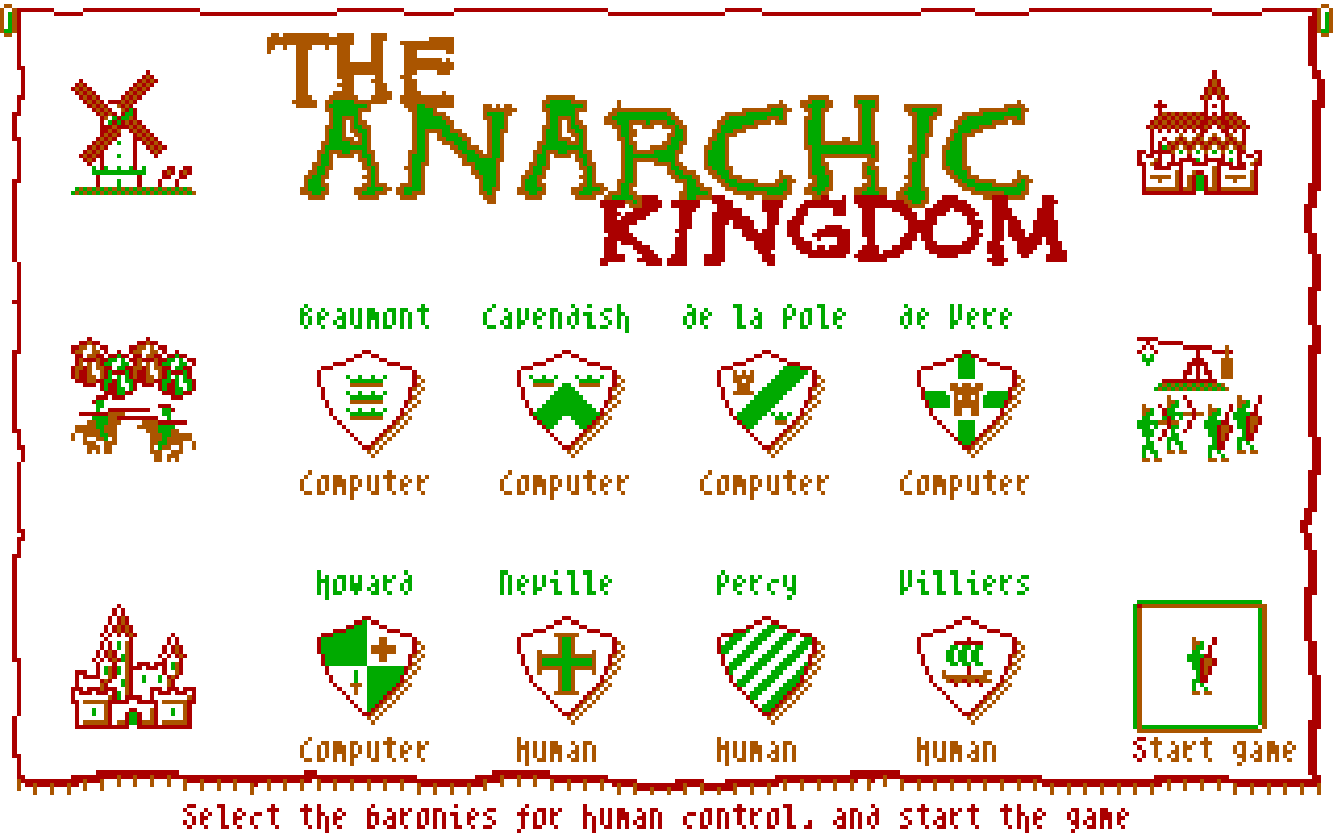
\includegraphics[width=\textwidth]{title}
  \caption*{The title screen.}
  \label{fig:title}
\end{figure*}

\begin{multicols}{2}
\noindent
The game starts on the title screen, which shows the shields of the eight baronies that will be fighting each other in the game. Above the shields are the baronies' names. Below the shields is the word ``Computer.'' This means that all the baronies are set to be computer controlled. Before starting, you need to decide how many humans are playing, and which baronies they will play.

Beaumont is initially highlighted with a square cursor. This can be moved around with the cursor keys, Pressing SPACE when highlighting a barony will flip it from ``Computer'' to ``Human'', or back again. This is how you will choose which baronies are human-controlled. When that is done, the cursor can be moved to ``Start game,'' and SPACE will begin the game.
\end{multicols}

%
% The Introduction
%

\pagebreak % because LaTeX is stupid
\section*{The Introduction}

\begin{figure*}
  \centering
  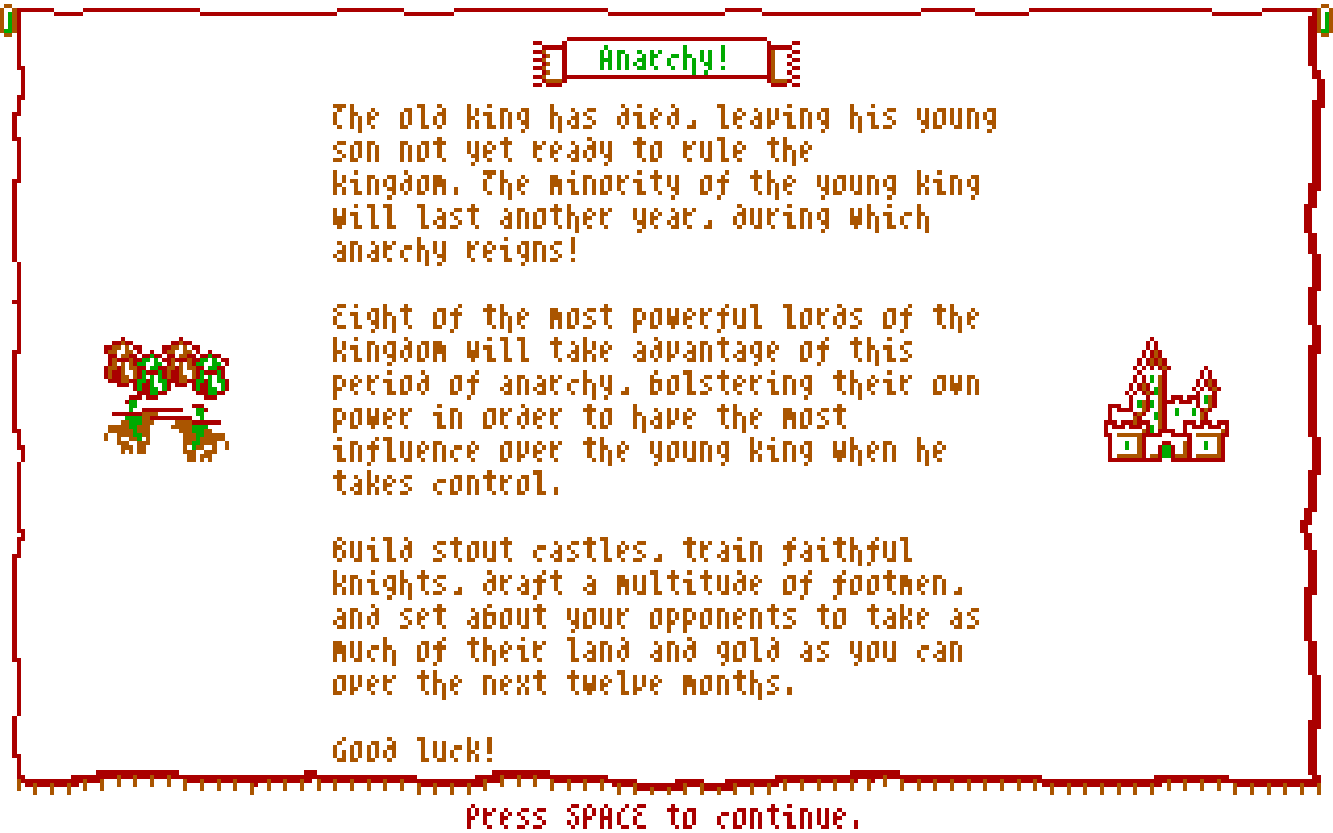
\includegraphics[width=\textwidth]{intro}
  \caption*{The introduction screen.}
  \label{fig:title}
\end{figure*}

\begin{multicols}{2}
\noindent
The first thing players will see is the text that introduces the game. This is the same text that introduces this manual, setting the scene of the game and telling players what they will be doing. The SPACE key will allow the game to begin in earnest and take the players either to the Main Menu (in a multiplayer game) or to the sole human player's barony (in a single-player game).
\end{multicols}

%
% The Main Menu
%

\pagebreak % because LaTeX is stupid
\section*{The Main Menu}

\begin{figure*}
  \centering
  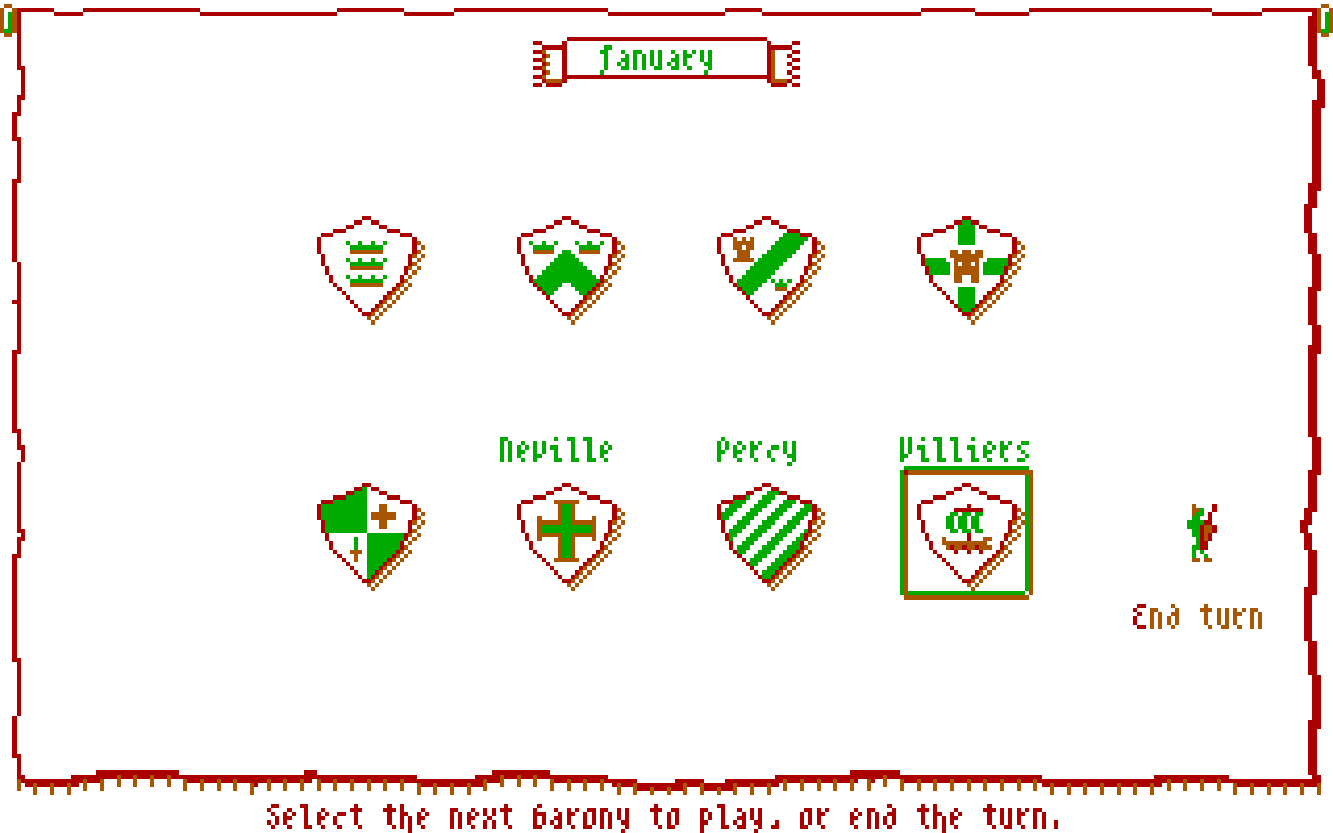
\includegraphics[width=\textwidth]{mainmenu}
  \caption*{The main menu.}
  \label{fig:title}
\end{figure*}

\begin{multicols}{2}
\noindent
In a multiplayer game, players will see the Main Menu at the start of each turn. Players can take their turn in any order, as their attacks and other orders are not put into effect till the turn ends. To select who gets to take their turn first, use the cursor keys to move the cursor to that player's shield and press SPACE. Note that only the human players have their baronies' names shown.

Once that player has taken their turn, the Main Menu will reappear for the other players to do likewise. When everyone has taken their turn, the last player can move the cursor to ``End turn'' and press SPACE. All the attacks and spending will then take place ready for the next turn.
\end{multicols}

%
% The Barony View
%

\pagebreak % because LaTeX is stupid
\section*{The Barony View}

\begin{figure*}
  \centering
  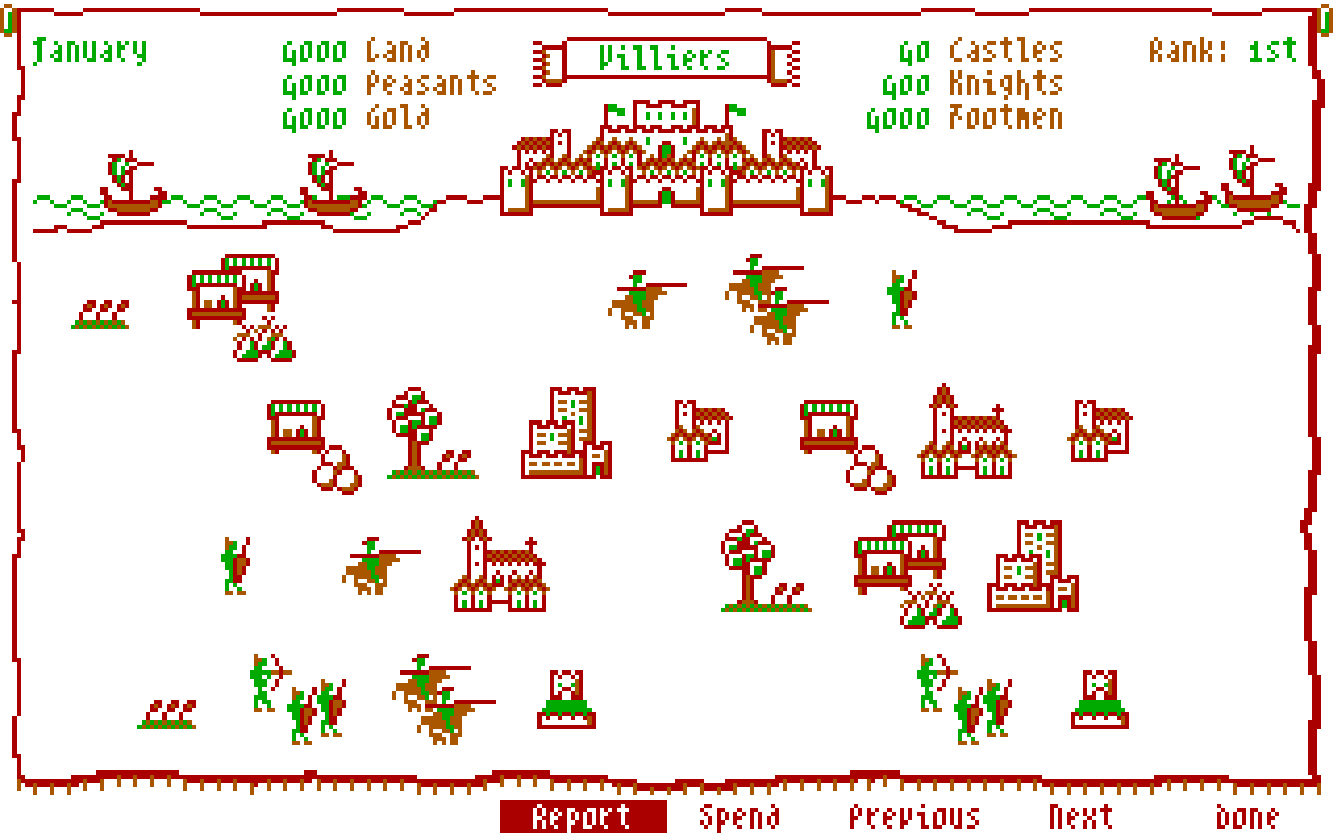
\includegraphics[width=\textwidth]{barony}
  \caption*{The barony view.}
  \label{fig:title}
\end{figure*}

\begin{multicols}{2}
\noindent
In a single-player game, the Main Menu will be skipped, and the player will be taken straight to their barony. In a multiplayer game, each player will begin their turn viewing their barony. The Barony View is the screen from which most of the game is played.

At the top of the screen is the hard information about the state of the barony. The title banner shows the barony's name. At the top left is the current month of the year, and the top right shows this barony's position in the rankings. In January, the baronies all start in joint first position---things can only go downhill from here.

Immediately left and right of the barony's name are the statistics. On the left are the economic statistics, and on the right are the military statistics. This would be a good place to explain them.

Land is the most important statistic, and is the number of square miles each barony covers. The rankings are by land area, and land also influences the number of peasants that a barony can support. The aim of the game is to be the barony with the most land when December's turn has been processed.

Peasants are the civilians who pay the taxes that support your military. They also provide the people to garrison your castles or to fight in your army as footmen. Each unit represents a ``parish'' of about 100 people. If the amount of land exceeds the number of peasants, this figure will rise as new peaseants move to your barony. If the amount of land falls short, then peasants will flee the barony to avoid famine and starvation. If there are no peasants, you can gather no tax!

Gold is the coin which pays for the building of castles and the training of knights. It also pays for the upkeep of all military units: 10 gold per turn to maintain a castle, 1 gold per turn to maintain a knight, and 1 gold per turn to maintain 5 footmen. If you haven't enough gold to pay your forces, they will start to desert you, so keep an eye on your income and expenditure!

Castles help to defend your barony against attacks. The more castles you have, the smaller the amount of land and gold that will be taken from you when your enemies come for you. It takes 100 gold to build a castle and 100 peasants to provide its garrison. A castle has the same fighting power as 10 knights or 100 footmen.

Knights are your main attack force. When sent against the other baronies, they will conquer land for you, and take control of your enemy's castles so you can put them for your own use. It takes 10 gold to train a knight. Knights do not take part in defence against enemy attacks. Ten knights are equivalent to a castle; one knight is equivalent to ten footmen in combat.

Footmen are a versatile force that you can use for attack or defence. When kept at home, 100 of them will be equivalent to a castle. When sent abroad, they will raze enemy castles to the ground and carry home the spoils as loot in gold. It takes 1 population to provide a footman, and 10 footmen are equivalent to a knight in battle.

Below all these hard numbers is a more graphical representation of the barony. The terrain on the horizon is different for each barony, to help you recognise them at sight. The capital city centred on the horizon varies in size according to the barony's position in the ranking. The various icons in the foreground are a rough representation of the economic and military state of the barony: windmills, trees and fields represent land; villages, towns and cities represent the peasants; markets of lesser or greater size reflect the gold. Castles, knights and footmen have their representation in the landscape too.

At the bottom of the Barony View is a menu. When viewing your own barony, the options are Report, Spend, Previous, Next, Done.

Report shows you the results of the previous turn's actions. In January there will be nothing to report, but in later months you will want to check this at the start of your turn to see how your attacks went, or if anyone else attacked you.

Spend allows you to use your resources (gold and peasants) to recruit military units. This is what you use to build castles, train knights and draft footmen. Spending is discussed in more detail later.

Next and Previous allow you to page through the other baronies to see how they are doing, and to select an enemy to attack.

When you are looking at barony other than your own, the Report and Spend options are absent but you see an Attack option instead. This allows you to send knights and footmen against the barony you are viewing.

Done ends the turn; in a multiplayer game it returns to the Main Menu for someone else to take their turn. In a single player game it goes straight to the Turn Processing view.
\end{multicols}

%
% Spending Your Resources
%

\pagebreak % because LaTeX is stupid
\section*{Spending Your Resources}

\begin{figure*}
  \centering
  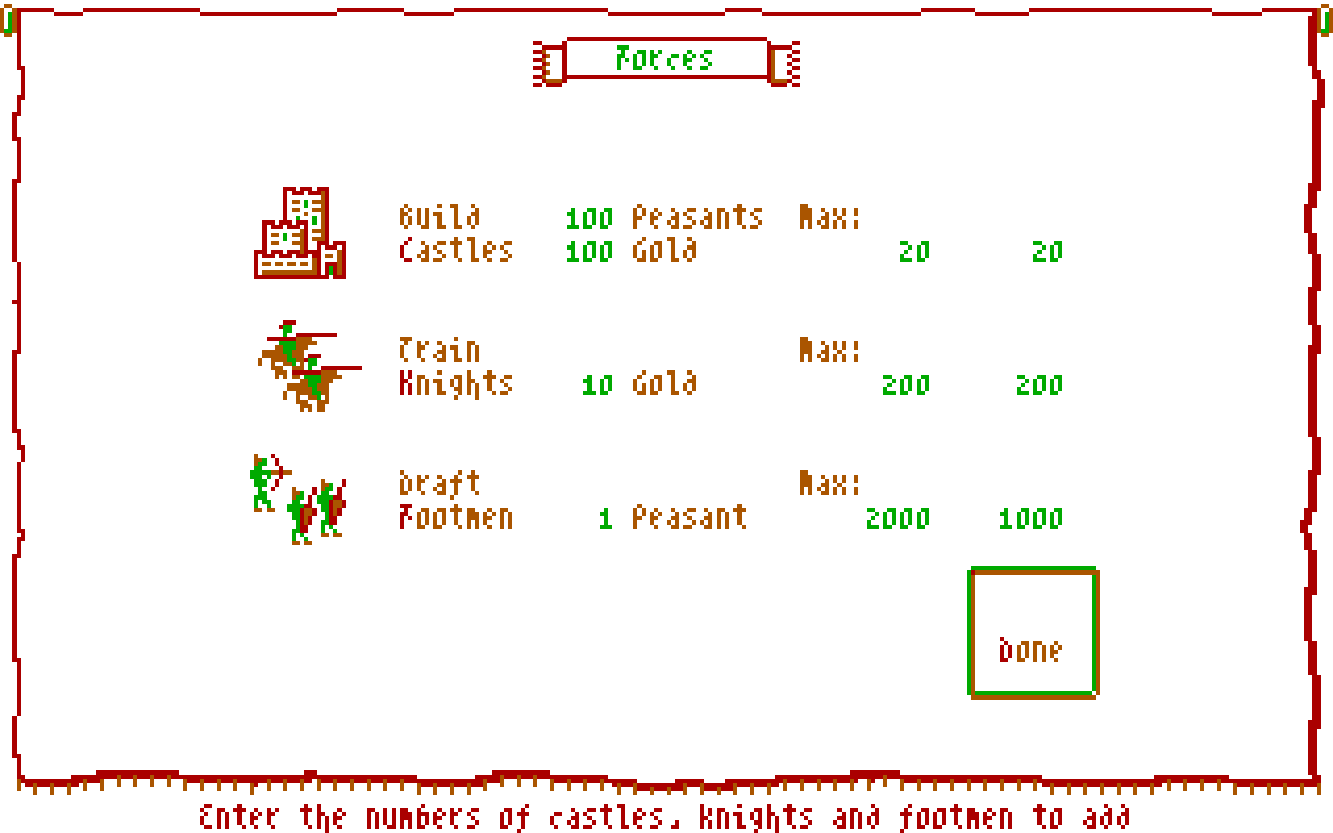
\includegraphics[width=\textwidth]{spend}
  \caption*{The spending screen.}
  \label{fig:title}
\end{figure*}

\begin{multicols}{2}
\noindent
When you choose the Spend option from your own Barony View, you are taken to another screen showing a table of military units: castles, knights and footmen. Here you can order new units to join your military in the next turn. The cursor begins by highlighting castles, but you can move it up and down with the cursor keys to select other units, or the Done option when you are finished.

The table shows how many peasants and/or footmen it takes for each unit, and also shows the maximum number that you can currently afford. These maximums are updated in real time; when you start to order castles, that leaves less gold for training knights and fewer peasants from which to draft footmen. The final column shows how many of each unit you are ordering; you can type the numbers or use the left and right cursor keys to increase and decrease the values.

When you are finished ordering units, moving the cursor down to the Done option and pressing SPACE will return to the barony view.

A word of warning: do not spend all your gold and draft all of your peasants in the same turn. If you do, you will have no gold left to pay for military units, and no peasants left to raise any more gold in tax. If you cannot afford to pay your new units, they will desert before you get to use them!
\end{multicols}

%
% Attacking the Enemy
%

\pagebreak % because LaTeX is stupid
\section*{Attacking the Enemy}

\begin{figure*}
  \centering
  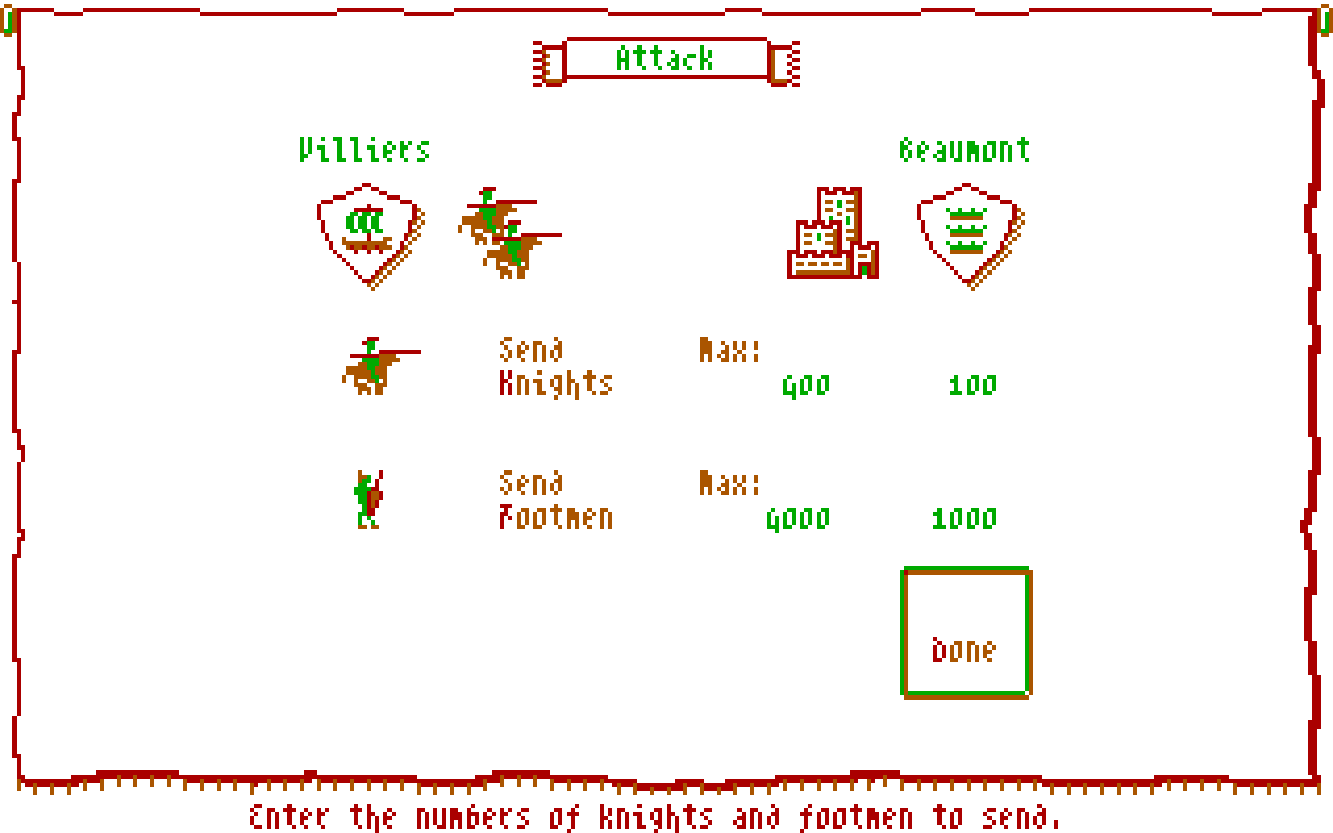
\includegraphics[width=\textwidth]{attack}
  \caption*{The attack screen.}
  \label{fig:title}
\end{figure*}

\begin{multicols}{2}
\noindent
When you choose to attack an enemy, you will see a table of military units. Here you can select the number of knights and footmen to send against this enemy. The table shows you the maximum in each case. The final column shows the number you are actually sending, and a cursor allows you to move up and down to select knights, footmen or the Done option.

To increase the number of knights or footmen you are attacking with, you can type the numbers or use the left and right cursor keys to increase and decrease the values. There are a few reasons why you might not want to send the maximum forces on an attack; firstly, you can attack more than one barony per turn, so you will keep some forces back to attack someone else. Secondly, you might keep some forces back to guarantee you have more to send next month. Thirdly, you might want to keep footmen back for defence against enemy attack.

After deciding how many knights and footmen to send against the current enemy, selecting the Done option will return to the Barony View.
\end{multicols}

%
% Viewing Reports
%

\pagebreak % because LaTeX is stupid
\section*{Viewing Reports}

\begin{figure*}
  \centering
  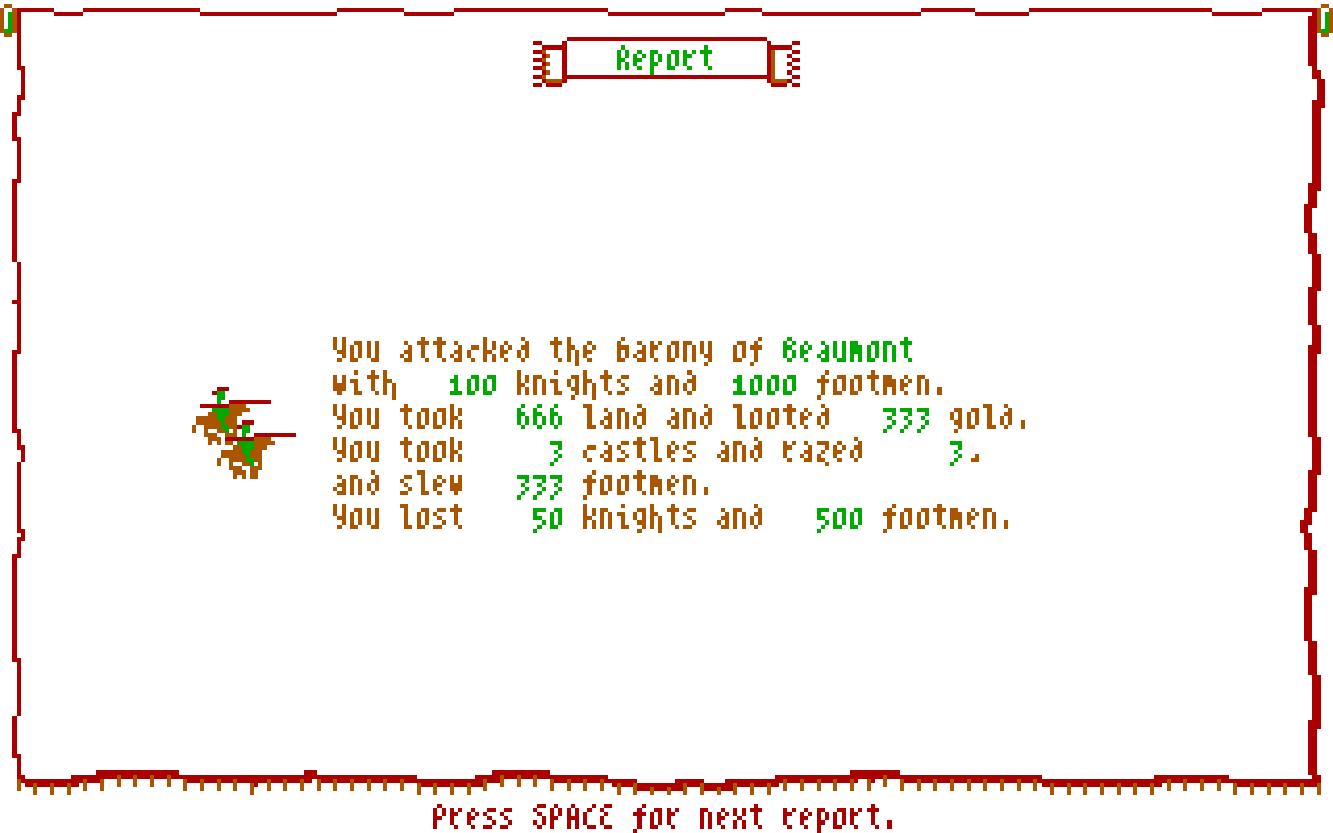
\includegraphics[width=\textwidth]{report}
  \caption*{One of the sections of the report screen.}
  \label{fig:title}
\end{figure*}

\begin{multicols}{2}
\noindent
From February onwards you will want to consult the Reports option to see the results of any attacks you launched the previous month, as well as any news of attacks sent against you. You will also want to see confirmation of the delivery of units you ordered the previous turn, and also news of population migration and tax income.

The reports view will present you reports on each of these, one at a time for easy digestion of the information. SPACE will advance through each report, after which the game will return to the Barony View. The month's reports can be requested as many times as you wish during your turn.
\end{multicols}

%
% Ending the Turn
%

\pagebreak % because LaTeX is stupid
\section*{Ending the Turn}

\begin{figure*}
  \centering
  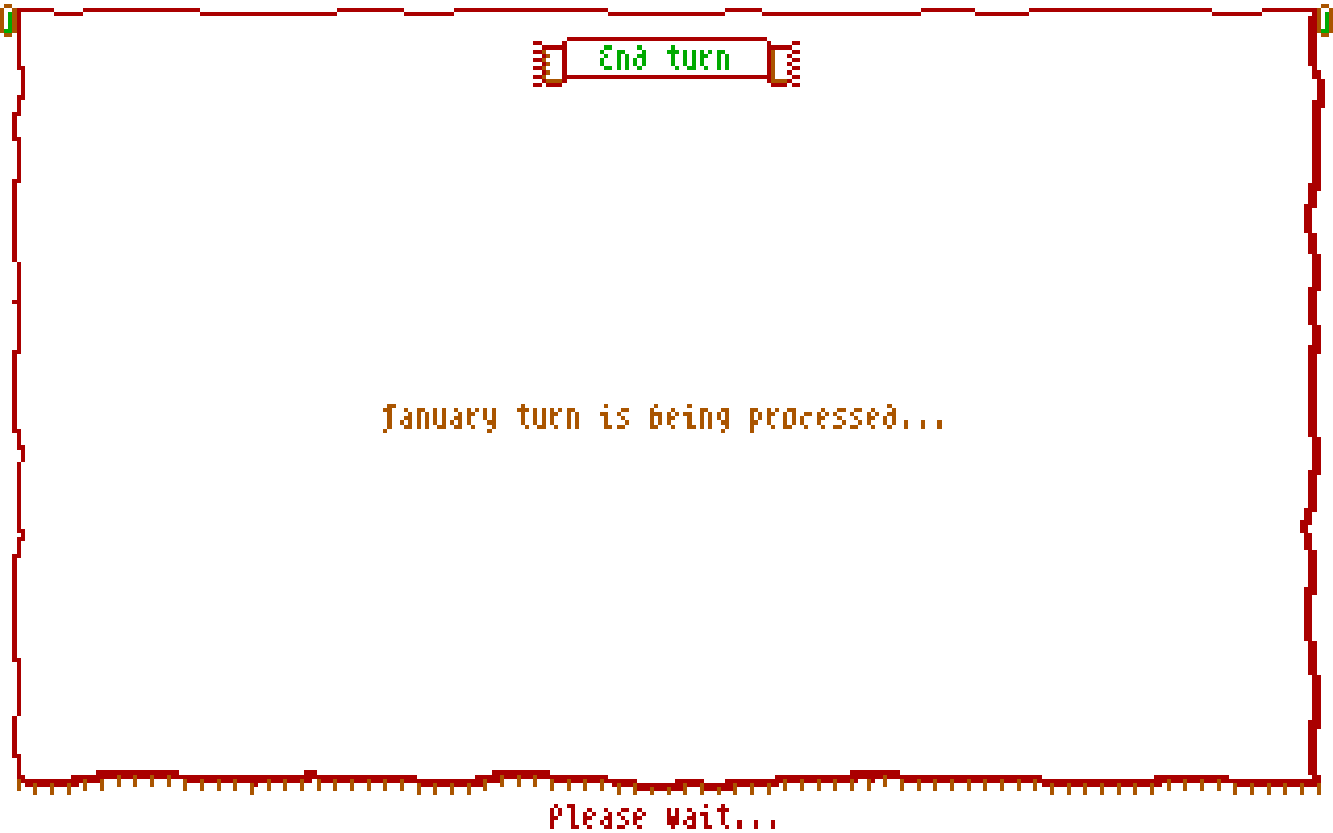
\includegraphics[width=\textwidth]{turn}
  \caption*{The end turn screen.}
  \label{fig:title}
\end{figure*}

\begin{multicols}{2}
\noindent
When all players have issued their orders, turn turn ends. The players will issue their orders, and then the turn will be processed. It might be useful to discuss now the order in which the various actions will happen.

First, gold and peasants required for the recruitments of the units the players ordered will be taken from the baronies. The units will not be delivered at this stage.

Then all the attacks will be conducted, simultaneously. This ensures that no player will be favoured or disadvantaged by their order in the barony list. Reports will be generated for all affected players to tell them how the battles went.

Then the peasants not drafted into the garrisons and armies will pay their taxes into the treasury. After the taxes are paid, new peasants will arrive, or peasants will flee if the barony cannot support them.

Then, military paid for earlier in the turn sequence will be delivered. The payment and delivery are separated like this in order that the peasants and gold required are not taken by the turn's battles, and that the units ordered do not take part in those battles. This helps to keep things somewhat predictable---especially in telling the players what units they should be able to afford for the next turn.

Finally, the upkeep of the military units is paid for, if possible, with desertion resulting if there are not the funds to pay them. This turn sequence tends to be very quick, so an artificial delay is introduced to allow players to read the "Processing turn..." message before it disappears.

If the turn being processed is December's turn, then the game passes to the End Game view where the players can see the final rankings. Otherwise, multiplayer games will return to the Main Menu while single-player games will return to the Barony View ready for the player's next turn.
\end{multicols}

%
% The End Game View
%

\pagebreak % because LaTeX is stupid
\section*{The End Game View}

\begin{figure*}
  \centering
  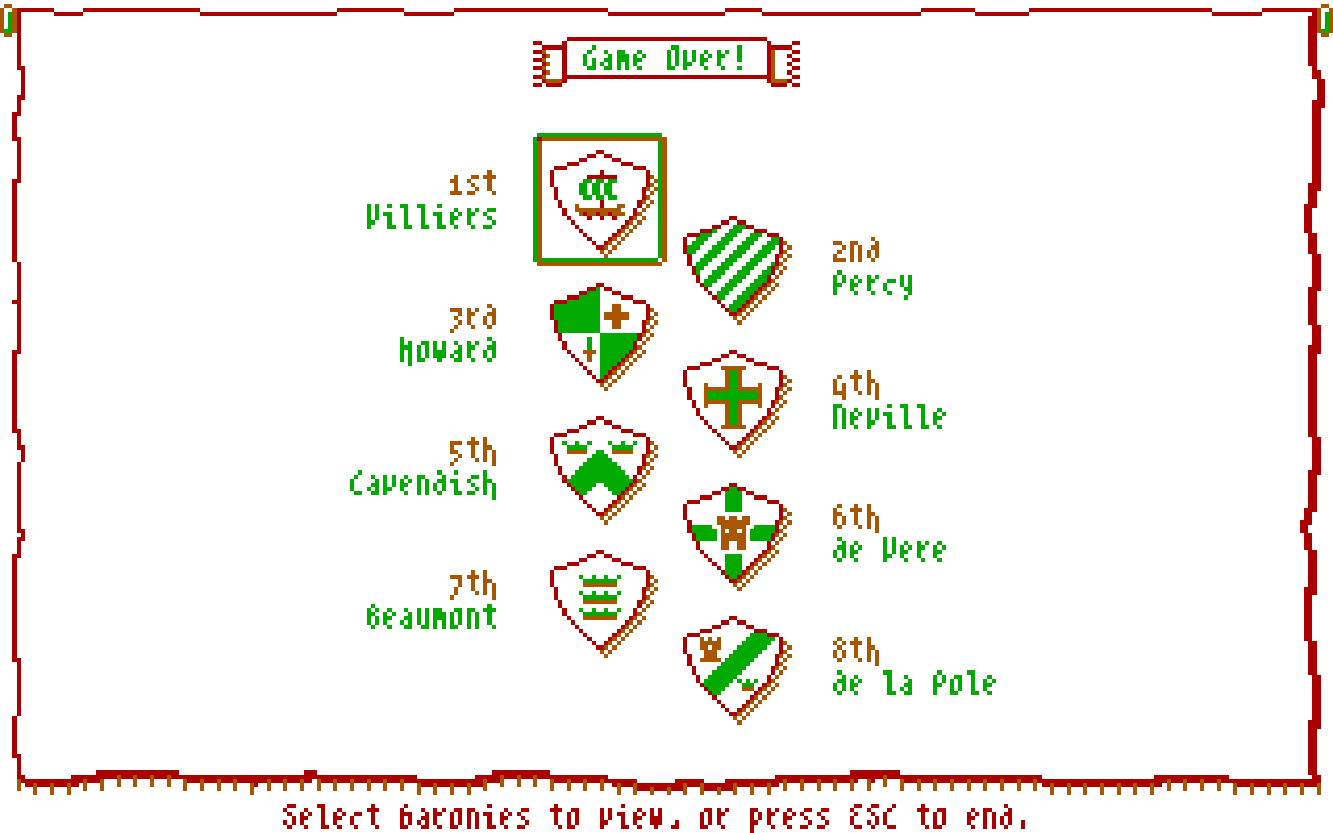
\includegraphics[width=\textwidth]{rankings}
  \caption*{The end game screen.}
  \label{fig:title}
\end{figure*}

\begin{multicols}{2}
\noindent
After December's turn is complete, players will see the final ranking. The baronies' shields are lined up vertically on the screen, with the winner at the top and the other baronies below in order of their ranking. A cursor highlights the last barony viewed, and can be moved with the cursor keys. Pressing SPACE will give a final view of the selected barony.

If viewing a human-controlled barony, a menu gives the option of viewing that barony's final Report. This allows players to see a detailed account of what happened on their last turn, if they wish. When viewing a computer-controlled barony, pressing SPACE returns the the End Game View.
\end{multicols}

%
% A Complete List of Controls
%

\pagebreak % because LaTeX is stupid
\section*{A Complete List of Controls}

\noindent
The Anarchic Kingdom is completely controlled from the keyboard. While the manual has explained the key controls needed as it went along, there are some alternatives. Please note that, apart from requiring the Esc key to leave the program, the game can be played entirely with the directional controls and SPACE for fire.

Esc: the final screen tells you explicitly that you can use Esc to quit there. But the key works anywhere in the game, so if you need to abort a game you can do so without resetting your cmputer.

1..8: in all screens that present a list of baronies, you can press this key to go to the relevant barony. The cursor will move there and the barony will be activated as if you had also pressed SPACE. Note that on the End Game screen, the keys do not correspond to the final rankings (because there can be two or more baronies jointly achieving the same position). The keys always refer to the baronies in the order they appear on the Start Game screen, i.e.

\begin{enumerate}
\item Beaumont
\item Cavendish
\item De la Pole
\item De Vere
\item Howard
\item Neville
\item Percy
\item Villiers
\end{enumerate}

Letters: options in a menu at the bottom of the screen can be selected by pressing their initial letter, instead of navigating to them with the cursor keys and pressing SPACE. Some options on the main screen (e.g. End turn) have letters highlighted to indicate you can use that letter to access that option.

ENTER: in nearly all cases the ENTER key can be used as an alternative to SPACE. This includes prompts that say ``press SPACE to continue.'' This makes it easier on some keyboards to navigate the game using the directional keys alone. On tabular screens where a value is being typed, ENTER will move down to the following row.

%
% Some Tips on Strategy
%

\pagebreak % because LaTeX is stupid
\section*{Some Tips on Strategy}

\begin{multicols}{2}
\noindent
The Anarchic Kingdom, as its name suggests, is a chaotic game. Players can plan their activities with care, but long-term planning is a waste of time because the state of the game can change so quickly. Instead, there is a strategy of ``weathering the storm,'' reacting to events in such a way as to improve one's position as much as possible from one turn to the next.

Players should make at least one attack every turn. No number of castles can prevent land being taken from you, they can only reduce the amount of land taken by a given attack. So in addition to defending, players should be making attacks in order to reclaim any land taken from them in the same turn as well as improving their own position. A barony that tries a purely defensive strategy will end up in a disastrous last place at the end of the game.

As mentioned in the section on Spending, it is not a good idea to recruit all your peasants and spend all of your gold on the same turn. This not only empties your coffers but also prevents you from refilling them in the next turn, leaving you with no gold to pay your military. So you must always leave something in your war chest, or leave some peasants to raise more gold.
\end{multicols}

%
% End of document
%

\null
\vfill
\begin{center}
\emph{http://dos.cyningstan.org.uk/}
\end{center}

\end{document}
